\chapter{Introduction}

We focus on investigation of existing pathways and not the creation of new ones (references?).

\chapter{Problem Definiton}

%Some types of cancer are suspected to either originate in or else being influenced by genetic disposition. Though human DNA has been examined and broken down to sequences of genes the meaning of most genes and their influence on each other is still unknown. The Cerberus application enables doctors to get an overview over patients' gene-expression data as well as clinical data like the history of the disease. It uses clustering techniques to provide information visualization, thereby allowing doctors to systematically search for coincidences. The aim of this thesis is to extend the application with a metabolic pathway module to take the connection between metabolic pathways and genes into account. 

\chapter{Related Work}

In this chapter first...

\section{Metabolic Pathway Visualization}

\subsection{Medical Pathways}

[Metabolism is defined in the book Metabolism at a glance and is cited in \citep{Bourqui2006}]

Metabolic networks are defined in \citep{Bourqui2006} as interconnected metabolic pathways.
[Write some more sentences about metabolic networks and why they are important to be investigated globally.]
Figure \stdref{gfx:RocheAppliedScience_MetabolicPathways_WallChart} shows a whole snapshot of a metabolic pathway.

\begin{figure}[ht]
\centering
\scalebox{0.43}{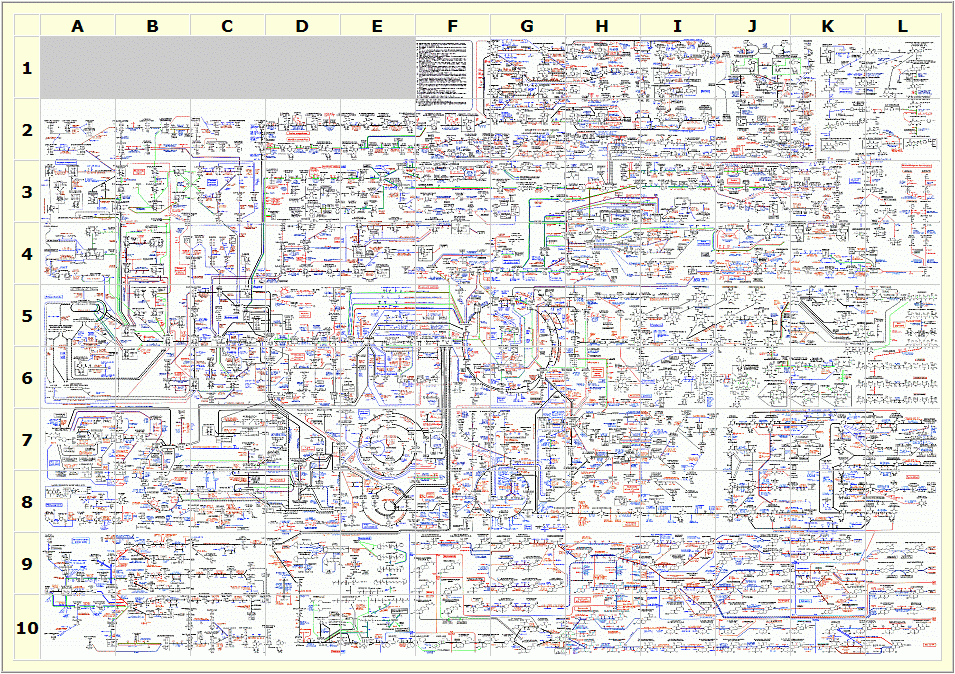
\includegraphics{gfx/RocheAppliedScience_MetabolicPathways_WallChart}} 
\caption[Roche Applied Science wall chart on metabolic pathways]{\textit{Roche Applied Science wall chart on metabolic pathways TODO Insert Reference}} 
\label{gfx:RocheAppliedScience_MetabolicPathways_WallChart}
\end{figure}

Metabolic pathways aim on modelling cellular functions in graphs. Basic building blocks of pathways are chemical compounds and enzymes. The chemical compounds act as substrates and products of chemical reactions. Enzymes catalyze these reactions by using substrates as input which is resulting in products. This process is described in LINK.

[Describe shortly the example methionine metabolism which is used throghout the thesis.]

\subsubsection{Definition}

\subsubsection{Layouting and Graph Drawing Algorithms}

Graph Drawing Algorithms are needed for layouting pathways dynamically.
Previous work on this issue was done by \citep{Becker2001}.

[Defintion of metabolic networks regarding graph theory is presented in \citep{Bourqui2006}.]
Propose a graph drawing algorithm for metabolic networks\citep{Bourqui2006}. They also address the problem of diplicate nodes
in different pathways.

\subsubsection{Pathway Visualization using Virtual Reality}

[Insert short definition of virtual reality - Judith bringt Referenz.]

\subsection{State-of-the-art Frameworks}

Brandes et al. propesed a 2.5D method to visualize differences accross pathways for different organisms\citep{Brandes2004}. This method enables the user to see evolutionary developments and relations amoung different species.

\minisec{PathwayExplorer [2005]}

The PathwayExplorer is able to map genes on enzymes in pathways from various databases.
Positive: Can handle all kind of identifiers (for example RefSeq, ...).
Negative: Needs time to map genes on pathways. The result are static PNG images.

\begin{figure}[ht]
\centering
\scalebox{0.43}{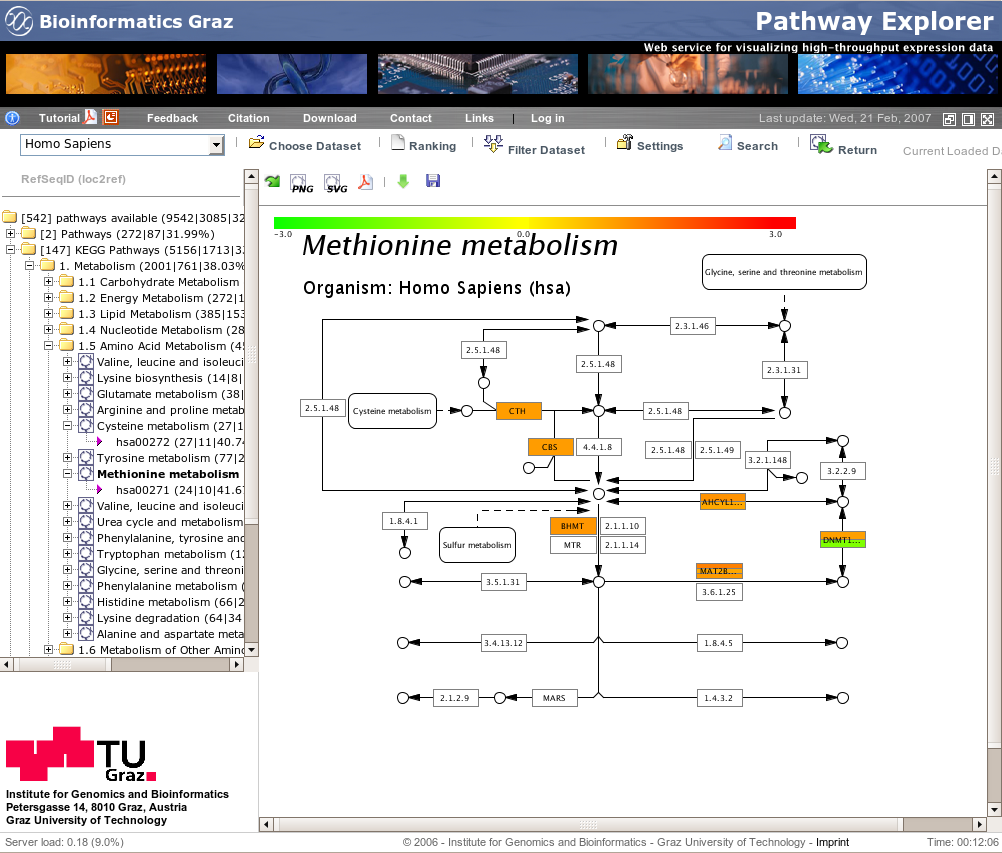
\includegraphics{gfx/screenshot_pathway_explorer}} 
\caption[PathwayExplorer]{\textit{PathwayExplorer}} 
\label{gfx:pathway_explorer}
\end{figure}

\section{Gene Expression Visualization}

\subsection{Gene-Expression Analysis}

Describe the Genome.
Human genome is sequenced since year by name -> Reference 
Describe how genes code enzymes (special proteins).
\subsection{State-of-the-art Frameworks}

http://www.genome.jp/kegg/expression/

\minisec{GeneSpring}
\minisec{Panther}

\section{Biomedical Databases}

Criterias for successful databases: 
Availability
Update rate / update process
ID Management (Unique Key)
Links to other databases
Software to access database (SOAP)
Documentation
Full data dump

\subsection{Gene centered databases}

\subsubsection{International Nucleotide Sequence Database Collaboration (INSDC)}

The INSDC is a collaborative network of DNA sequence databases that consists of three major members:
\begin{itemize}
 \item \textbf{GenBank:} \\
 GenBank is a part of the National Center for Biotechnology Information (NCBI) which is intergrated in the United States National Library of Medicine (NLM). NLM belongs to the National Institutes of Health (NIH) that is self-described as the focal point for medical research in the United States.
 \item \textbf{European Molecular Biology Laboratory (EMBL):} \\
 EMBL
 \item \textbf{DNA Data Bank of Japan (DDBJ)} \\
\end{itemize}

INSERT table with current data sets in various databases
Number of genes, proteins, enzymes.

\subsubsection{Entrez}

\subsubsection{Gene Ontology (GO)}

\subsection{Pathway centered databases}

\subsubsection{Kyoto Encyclopedia of Genes and Genomes (KEGG)}

The Kyoto Encyclopedia of Genes and Genomes (KEGG)\footnote{http://www.genome.jp/kegg/} is a biomedical resource that started its online service in 1995 and belongs to the Japanese GenomeNet.

Provide 140 metabolic pathways for over ?? organisms.

KEGG pathways are represented by graphs which are layouted by hand and stored in static images (reference?). [Images are generated, how?]

In the graph enzymes are visualized by rectangular nodes and compounds are modelled by small circles. Round rectangular nodes depict linked pathways. This circumstance points to the fact that a pathway is only an artificial subset of a huge complex network. 

When a cellular function is valid throughout different organisms it is called strongly preserved. These general pathways are stored in the KEGG database as reference pathways. Each reference pathway can then be specialized for a specific organism. Figure BLA shows the methionine metabolism for home sapiens. Light green color coded enzymes depict proteins where the generating genes are known. 

\subsubsection{BioCyc}
\subsubsection{ExPASy Molecular Biology Server}

\begin{figure}[ht]
\centering
\scalebox{0.4}{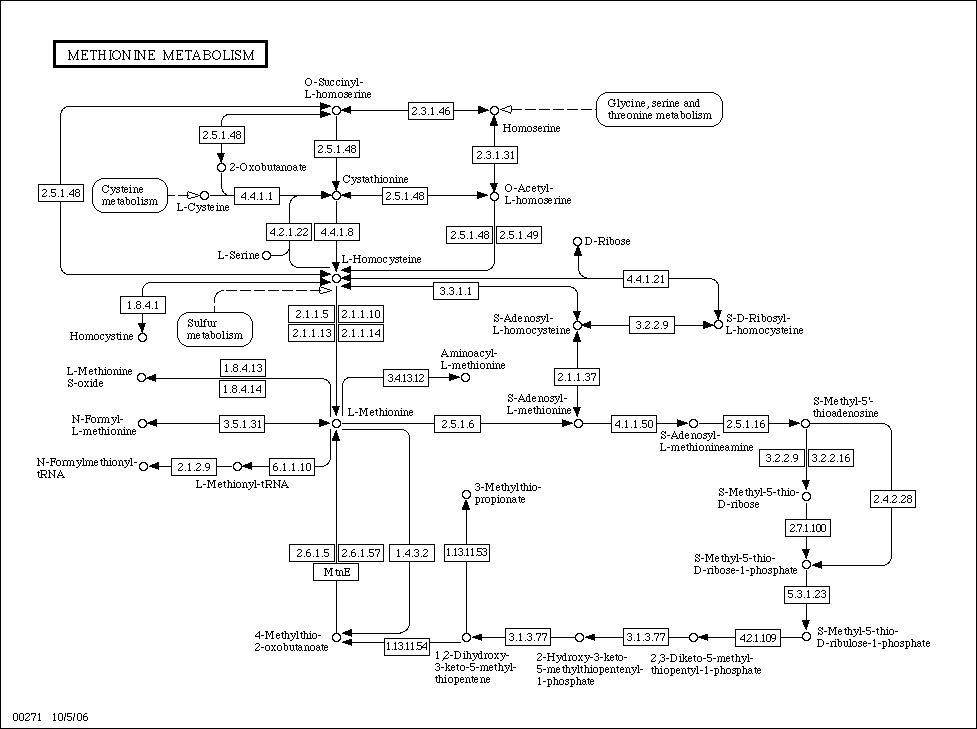
\includegraphics{gfx/KEGG_methionine_metabolism_271_reference_pathway}} 
\caption[KEGG methionine metabolism reference pathway]{\textit{KEGG methionine metabolism reference pathway}} 
\label{gfx:KEGG_methionine_metabolism_271_reference_pathway}
\end{figure}

\begin{figure}[ht]
\centering
\scalebox{0.4}{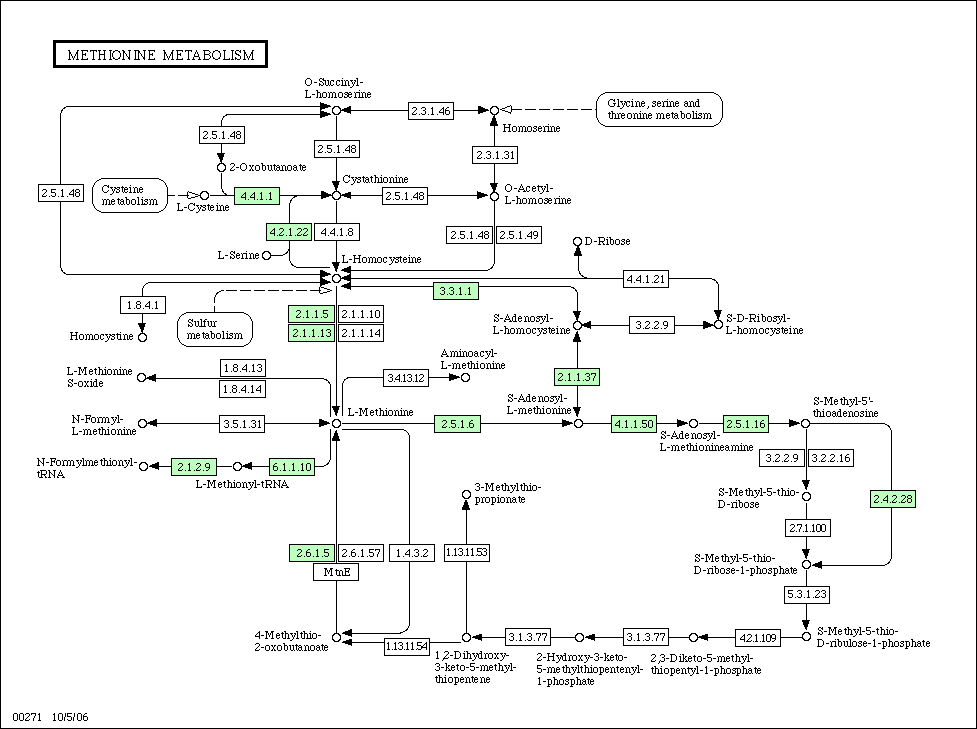
\includegraphics{gfx/KEGG_methionine_metabolism_271_pathway_hsa}} 
\caption[KEGG methionine metabolism pathway for home sapiens]{\textit{KEGG methionine metabolism pathway for home sapiens}} 
\label{gfx:KEGG_methionine_metabolism_271_pathway_hsa}
\end{figure}

\subsection{Biomedical Identification Numbers}

During the last decade biochemical database projects sprang up like mushrooms. Some projects has proven their value and achieved to manifest themeselves inside the community. Each database project introduced their own identification numbers for genes, proteins, nucleotids, etc. The obvious problem is how to map these data and interconnect them among the misscellaneous databases. 
There were many attempts over the time to get the issue under control.

The nomenclature for enzymes become widely accepted. The Nomenclature Committee of the International Union of Biochemistry and Molecular Biology (NC-IUBMB) agreed on the Enzyme Commission number (EC number). For details see http://www.chem.qmul.ac.uk/iubmb/enzyme/.

In the case of genes unique identifiers are much more silvered.

Identification Number

\section{Information Visualization Methods}

\subsection{2D vs. 3D}

\subsection{Multiple Views}
\subsection{Focus + Context}
\subsection{Linking \& Brushing}
\subsection{Semantic Zooom}

\section{Application of Gene-Expression Data onto Metabolic Pathways}

%Nochmal in implementation/results

\chapter{System Architecture}

\begin{figure}[ht]
\centering
\scalebox{0.4}{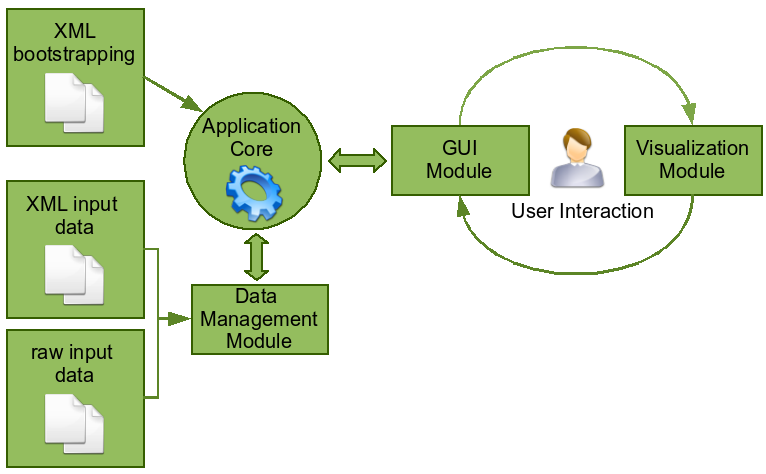
\includegraphics{gfx/application_block_chart}} 
\caption[Application block chart]{\textit{Application block chart}} 
\label{gfx:application_block_chart}
\end{figure}

\section{Overall Design}
%\section{Data Management}
\section{Pathway Data Management}

From information point of view metablic pathways are graphs. The nodes are enzymes and compounds. The edges can be differenciated in relations and reactions.

\begin{figure}[ht]
  \centering
    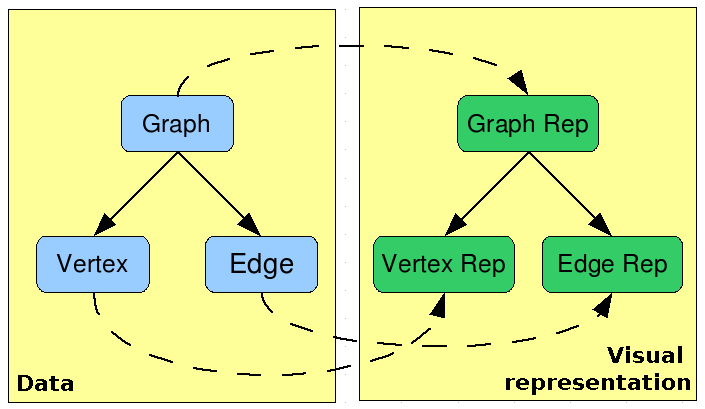
\includegraphics[width=0.5\linewidth]{gfx/model_view_data_diagram}
  \caption{Model abstraction into data and visual representations}
  \label{fig:model_view_data_diagram}
\end{figure}

[The problem description why this solution is needed is very good described in \citep{Bourqui2006}.]

\begin{figure}[ht]
  \centering
    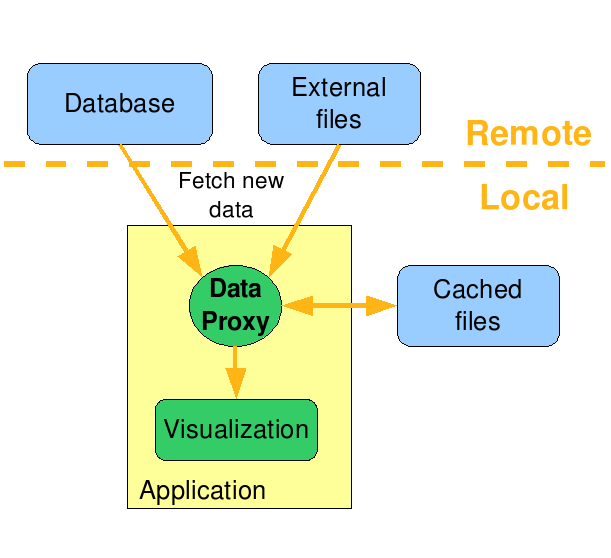
\includegraphics[width=0.5\linewidth]{gfx/data_block_diagram_new}
  \caption{Data block diagram showing the data loading process}
  \label{fig:data_block_diagram}
\end{figure}

%\subsection{Set / Storage / Virtual Array}

%Referenz auf Michaels Thesis

\section{Graphical User Interface (GUI)}

\section{Data Update Mechanism}

%Selection handling included 

\section{Enzyme-Gene Mapping (??)}

\begin{figure}[ht]
\centering
\scalebox{0.35}{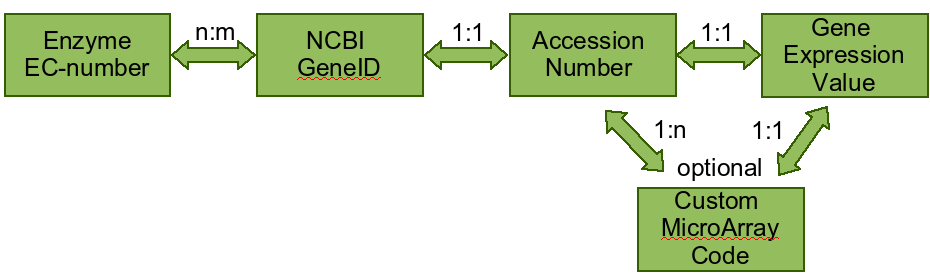
\includegraphics{gfx/enzyme_gene_mapping}} 
\caption[Enzyme-Gene Mapping]{\textit{Enzyme-Gene Mapping}} 
\label{gfx:enzyme_gene_mapping}
\end{figure}

\chapter{Implementation}

\section{Used Technologies}
\subsection{Standard Widget Toolkit (SWT)}

SWT\footnote{http://www.eclipse.org/swt/} is an open source library for creating graphical user interfaces. The project was initiated 2001 by IBM under within the scope of the Eclipse framework\footnote{http://www.eclipse.org}. In contrast to the standard Java toolkits like the Abstract Widget Toolkit (AWT) and Swing took the SWT designer an approach which is closer to the native operating system widgets. This results in a better performance and a native look of the widgets.

\subsection{JOGL}

Java OpenGL library\footnote{https://jogl.dev.java.net/}

%\subsection{OpenGL integration in Java}
\subsection{JGraph}

\section{Data Loading}

TODO describe:
XML loading
XML files are provided by KEGG.
Also a SOAP interface for KEGG information retrieval exists. Due to the fact that real-time behaviour of the application is in the main focus the SOAP alternative was too slow.

Problem of double data keeping. 

\section{Visualization Techniques}

In the upcoming section used visualization techniques are described and how they were realized.

\subsection{2D Pathway Implementation}

\begin{figure}[ht]
  \centering
    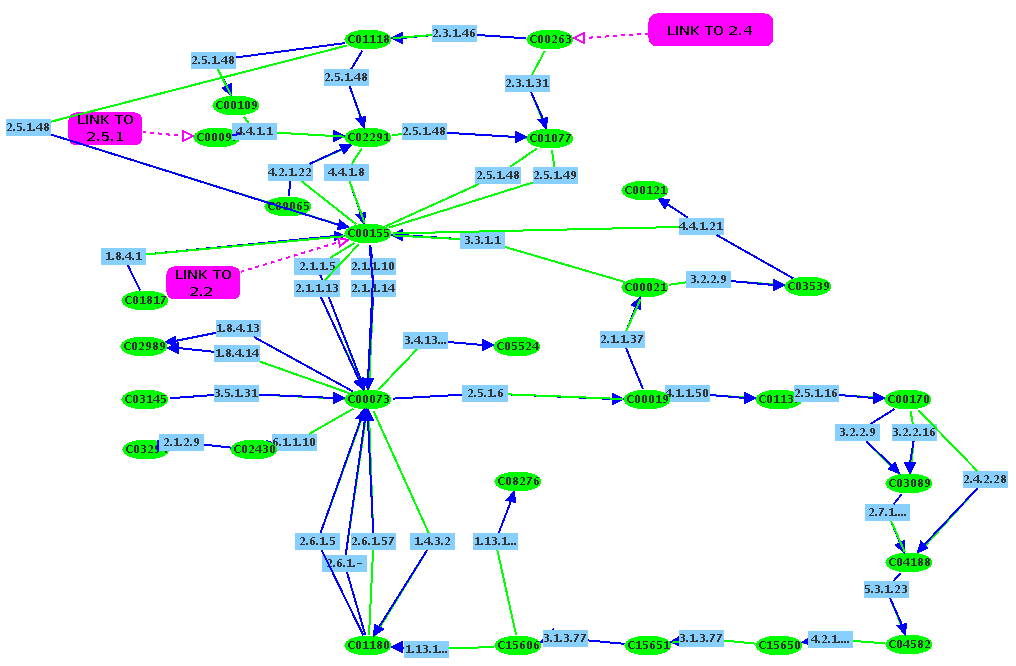
\includegraphics[width=0.7\linewidth]{gfx/sample_pathway_jgraph}
  \caption{Sample pathway without any layouting modification.}
  \label{fig:sample_pathway_jgraph}
\end{figure}

\begin{figure}[ht]
  \centering
    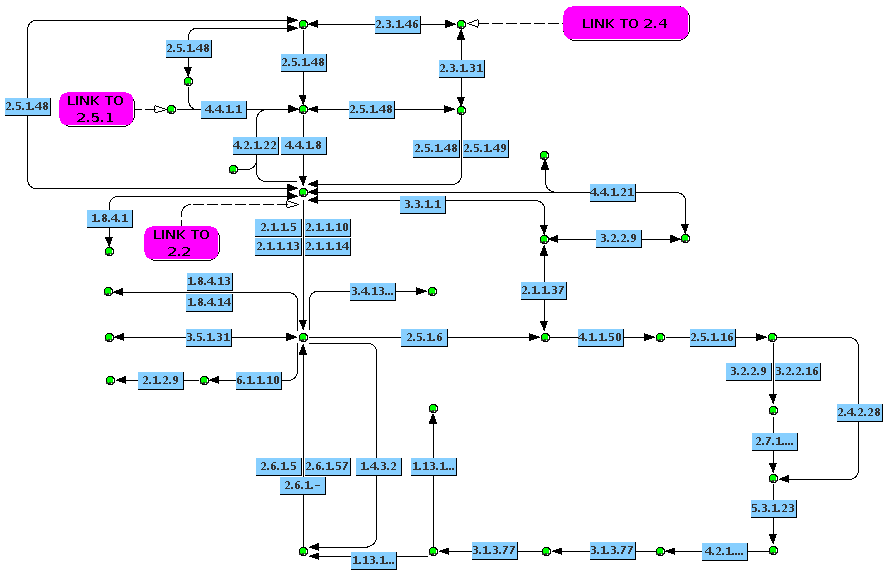
\includegraphics[width=0.7\linewidth]{gfx/sample_pathway_jgraph_background}
  \caption{Sample pathway with background texture overlay.}
  \label{fig:sample_pathway_jgraph_background}
\end{figure}

\subsubsection{Pathway Switching}

Pathways are linked to related pathways. Therefore we implemented fast switching by simply clicking on the pathway node.

\subsubsection{Hierarchical Pathways}

KEGG added two abstraction levels above the metabolic pathways. The pathways are categorized in 10 groups which represent the highest layer. The middle level...
\stdref{gfx:KEGG_abstraction_chain} shows the three KEGG abstraction levels. 
In the webbased KEGG version each abstract level has a imagemap in the back. In the imagemap rectangular portions are defined and provided with a hyperlink to next layer below. We use the same mechanism for linking pathways between abstraction levels. In contrast to KEGG we store the imagemap information in XML which is parsed at bootstrapping. During runtime when a mouse event is triggered on the 2D pathway the clicked position is checked if it is contained in a predefined area. If a positive match is found the link for this area is returned and the requested next layer map can be loaded.

\begin{figure}[ht]
\centering
\scalebox{0.35}{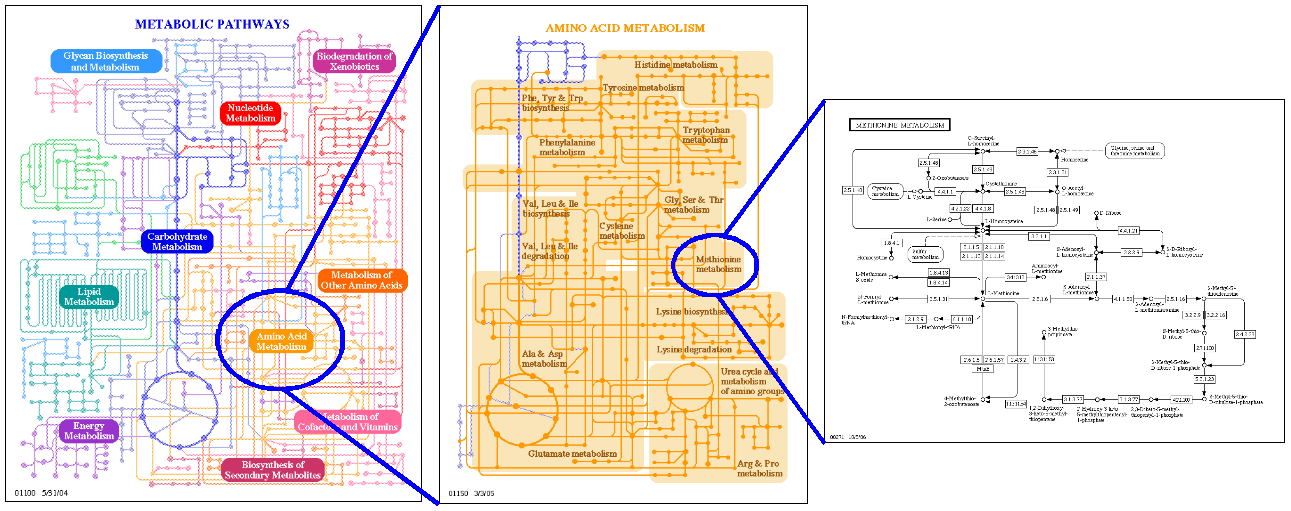
\includegraphics{gfx/KEGG_abstraction_chain}} 
\caption[KEGG abstraction chain]{\textit{KEGG abstraction chain}} 
\label{gfx:KEGG_abstraction_chain}
\end{figure}

\subsubsection{Neighborhood Visualization}

In graphs where the layout aims on the positioning of nodes and edges to circumvent intersections neighborhood visualization takes an important role. 
Cyclic charakter

Modified Breadth-First-Search (BFS) Algorithm.

\begin{figure}[ht]
  \centering
    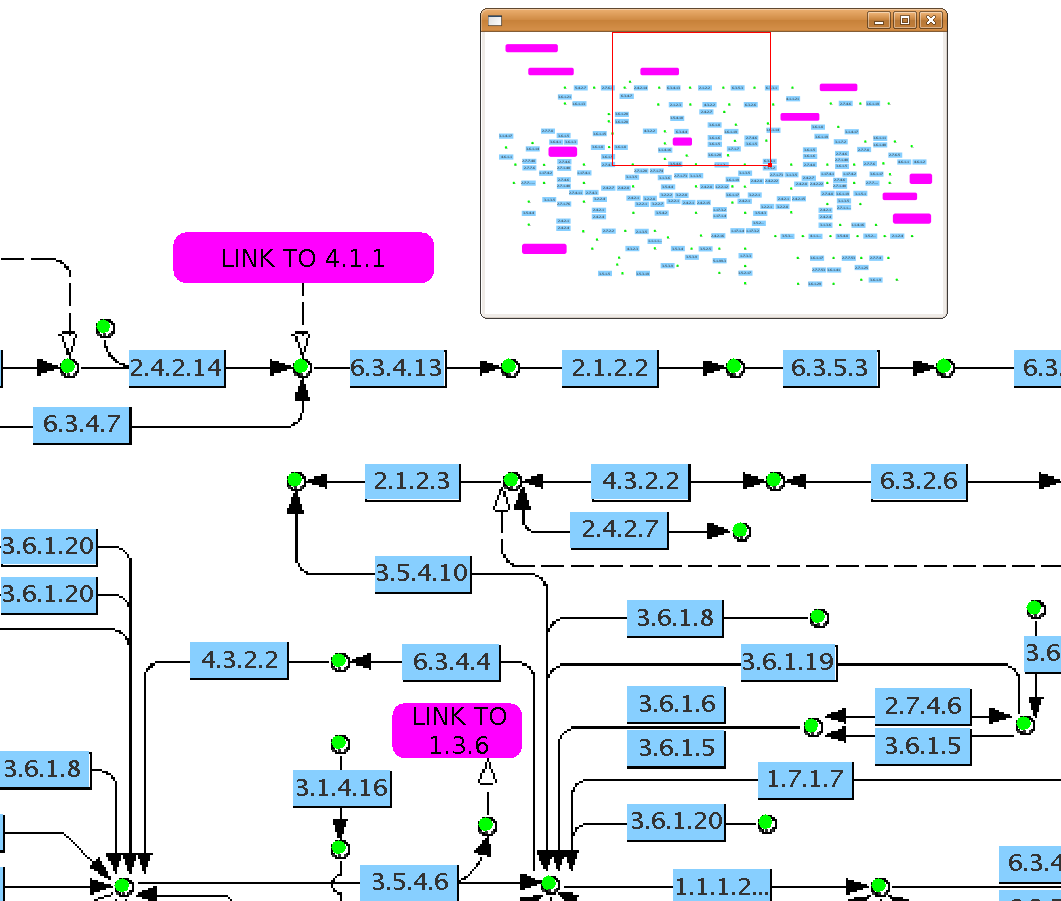
\includegraphics[width=0.5\linewidth]{gfx/overview_method}
  \caption{Portion of a sample pathway that can be interactively selected in the overview map.}
  \label{fig:overview_method}
\end{figure}

\subsection{OpenGL Pathways}

\begin{figure}
  \centering
    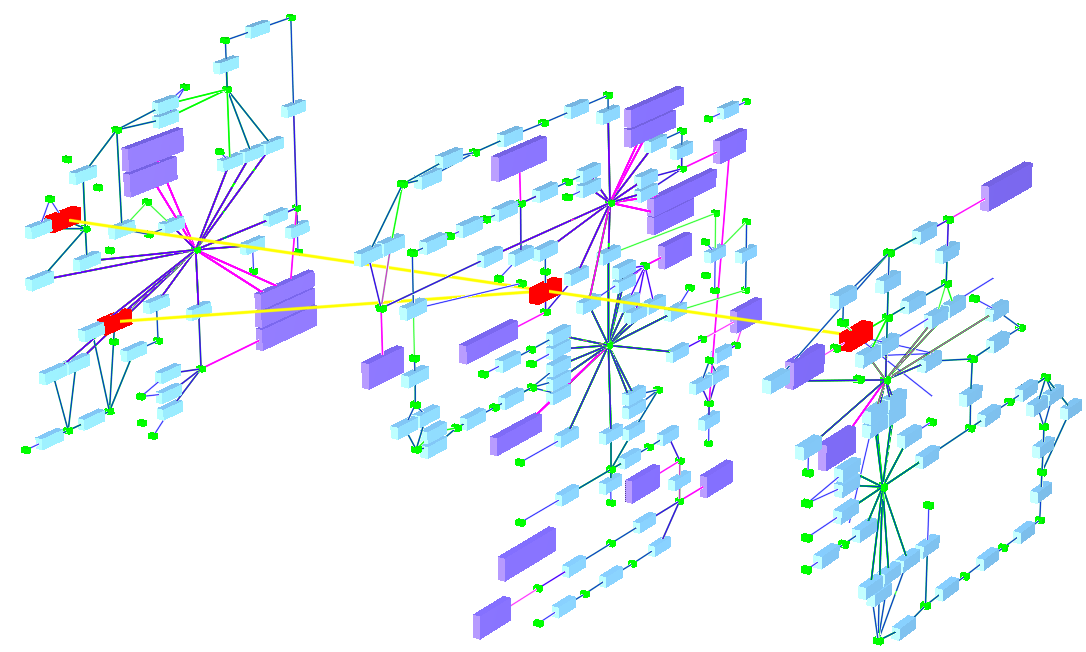
\includegraphics[width=0.7\linewidth]{gfx/opengl_layered_pathway_without_texture}
  \caption{2.5-D OpenGL layered pathway with a user selection}
  \label{fig:opengl_layered_pathway_without_texture}
\end{figure}

\subsubsection{Pathway Texture Overlay}

\begin{figure}[ht]
  \centering
    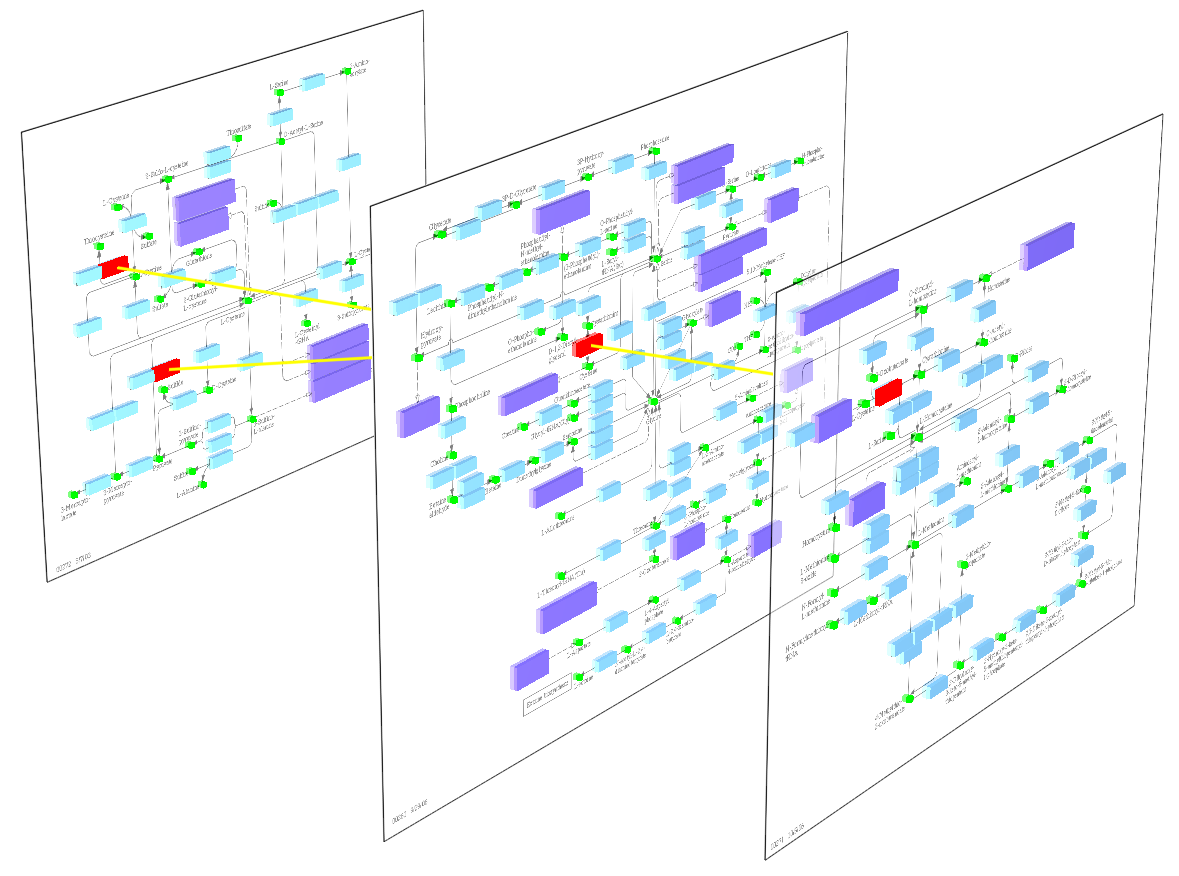
\includegraphics[width=0.7\linewidth]{gfx/opengl_layered_pathway}
  \caption{2.5-D OpenGL layered pathway with a blended texture overlay. The node in the middle layer is picked by a mouse-click event. Identical nodes in dependent graphs are interactively highlighted and connected to the selected one.}
  \label{fig:opengl_layered_pathway}
\end{figure}

\subsubsection{Pathway Linking}


\subsubsection{Pathway Element Picking}


\subsubsection{Hierarchical Display Lists}

\citep{Shreiner2005}

\subsubsection{Layered Pathways}

\subsubsection{Panel View}

\chapter{Results}

%Reflections from Zatloukal

\chapter{Conclusions}

\chapter{Future Work}

\index{bla}


